\documentclass{article}
\usepackage[utf8]{inputenc}
\usepackage[spanish]{babel}
\usepackage{listings}
\usepackage{graphicx}
\graphicspath{ {images/} }
\usepackage{cite}

\begin{document}

\begin{titlepage}
    \begin{center}
        \vspace*{1cm}
            
        \Huge
        \textbf{Taller de Memoria}
            
        \vspace{0.5cm}
        \LARGE
        Informática II
            
        \vspace{1.5cm}
            
        \textbf{Santiago Alejandro Sepulveda Palacio }
        \textbf{CC. 1022097969 }  
        
        \vspace{1.5cm}
        \textbf{Profesor: Augusto Enrique Salazar Jimenez }
        \vfill
            
        \vspace{0.8cm}
            
        \Large
        Despartamento de Ingeniería Electrónica y Telecomunicaciones\\
        Universidad de Antioquia\\
        Medellín\\
        Septiembre de 2020
            
    \end{center}
\end{titlepage}

\tableofcontents
\newpage

\section{Introducción.}

En este articulo se verán las definiciones de memoria de un computador y algunos diferentes tipos de memorias que existen, de igual forma se tratará de explicar como se gestiona la memoria dentro de un computador y por que es importante la rapidez de éstas.  

\section{Defina que es la memoria del computador.}

La memoria de un computador es un dispositivo que almacena datos  temporalmete para permitirle a un microprocesador (otro dispositivo de la computadora) realizar tareas o instrucciones ordenadas por el usuario. Este dispositivo tiene un determinado espacio para perimitirle trabajar al microprocesador de forma más veloz y asi evitar ir al disco duro que es mucho más lento. La memoria tiene diferentes espacios que se van ocupando para realizar estas diferentes tareas pero que tambien se van liberando a medida que ya se han finalizado éstas para ahorrar espacio de memoria y asi optimizar los procesos llevados a cabo.

\vspace{0.5cm}

A continuación se presenta una ilustración de una memoria RAM Figura
(\ref{fig:memoriaRAM})
\begin{figure}[h]
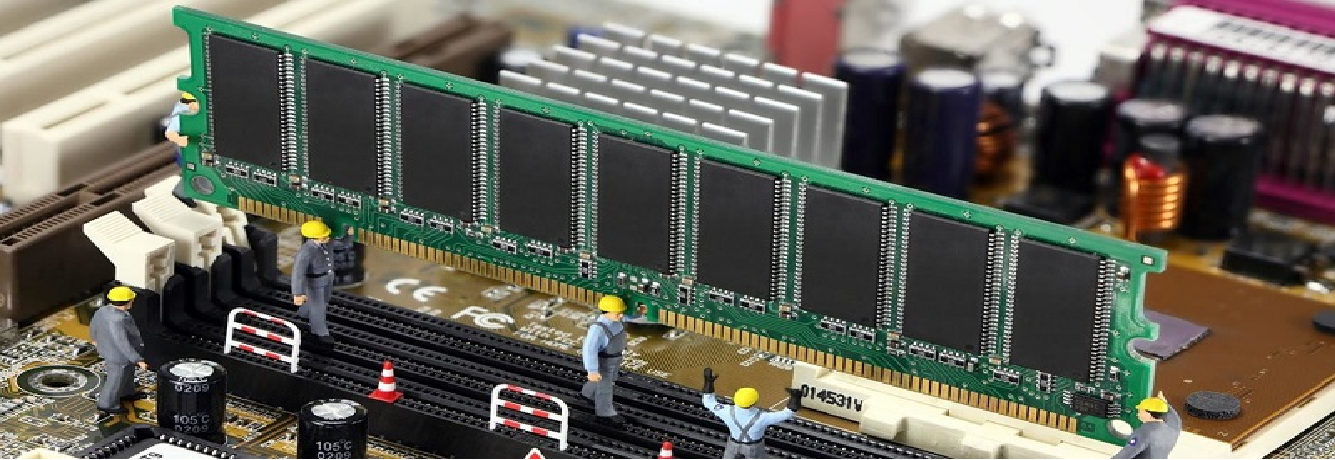
\includegraphics[width=4cm]{memoriaRAM.png}
\centering
\caption{Memoria RAM}
\label{fig:memoriaRAM}
\end{figure}


\section{Mencione los tipos de memoria que conoce y haga una pequeña descripción de cada tipo.}

Memoria RAM. Dispositivo que contiene diferentes espacios de memoria que son usados de forma temporal para almacenar datos para que el  micoprocesador pueda realizar tareas e instrucciones.

\vspace{0.5cm}

Memoria caché. Es un tipo de memoria situada dentro del microprocesador que se utiliza para almacenar los datos e instrucciones con los que el microprocesador trabaja más seguido y así evitar ir a la memoria RAM siendo más velóz. 

\vspace{0.5cm}

Disco duro. Es un dispositivo de memoria que almacena los datos más importantes de la computadora como sistema operativo, programas y archivos. Estos datos una vez guardados siempre permanecen almacenados y no son liberados. \cite{GCFglobal}

\vspace{0.5cm}

A continuación se presenta una ilustración de un disco duro Figura

(\ref{fig:DiscoDuro})
\begin{figure}[h]
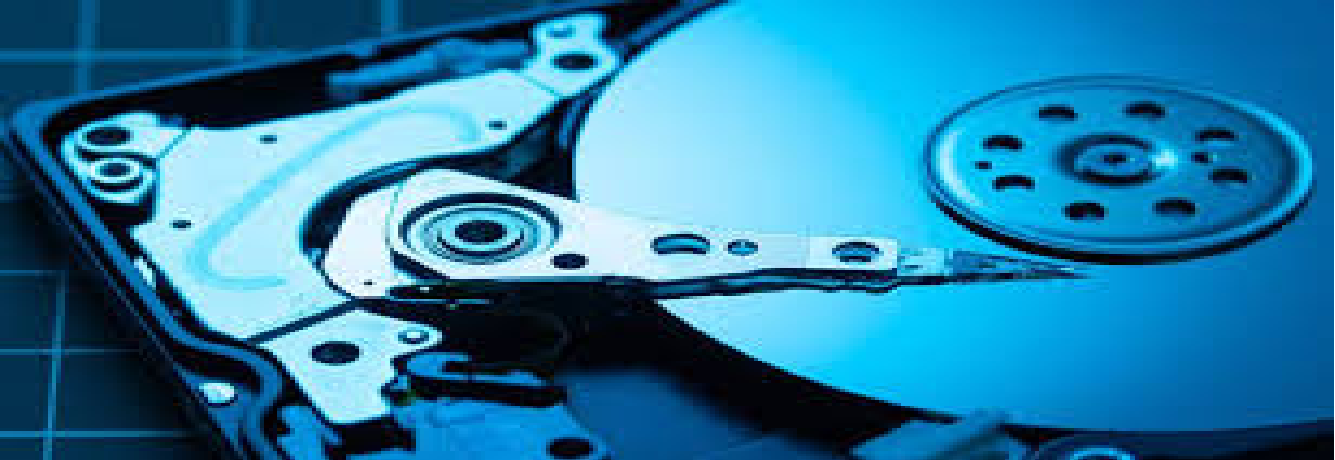
\includegraphics[width=4cm]{DiscoDuro.png}
\centering
\caption{Disco Duro}
\label{fig:DiscoDuro}
\end{figure}

\section{Describa la manera como se gestiona la memoria en un computador.}

\vspace{0.5cm}

Todo inicia desde el usuario quien da una instrucción de abrir un programa por ejemplo que se encuentra almacenado en el disco duro de la computadora, esta instruccion viaja hasta la memoria y se ubica en un espacio de memoria esperando a que esa instruccion sea procesada. El microprocesador recibe un aviso de que en un espacio de memoria hay una instrucción y procede a ir a ese espacio de memoria donde está dicha instrucción, la misma es leída por el microprocesador indicáncole que debe abrir un programa ubicado en el disco duro. luego la orden se elimina tanto del procesador como de la memoria, para que dicho espacio no sea ocupado por algo que ya ha sido utilizado. De esta manera el procesador le envía la orden a un controlador especial ubicado motherboard. Dicho controlador toma el programa que está almacenado en el disco duro y la lleva hasta la memoria, colocándola en un espacio vacío de la misma para poder trabajar con el. Y por último, el microprocesador comienza a poner en operación el programa una vez ubicado en la memoria.

\section{¿Qué hace que una memoria sea más rápida que otra? ¿Por qué esto es importante?.}

\vspace{0.5cm}

La velocidad de los módulos de memoria depende de la velocidad del bus, o sea las pistas del circuito impreso de la motherboard por la que viaja la información de un dispositivo a otro, y más concretamente de la velocidad del reloj del bus que une la memoria con el microprocesador. \cite{MemoriaDelComputador}

\vspace{0.5cm}

la rapidez de una memoria es importante por que la velocidad de la memoria RAM determinará la velocidad a la que la CPU pueda procesar los datos. Cuanto mayor sea la calificación del reloj de la RAM, más rápido podrá el sistema leer y escribir información en la memoria.\cite{TarjetasGraficasPC}

\vspace{0.5cm}

Toda la memoria RAM estándar se clasifica a una velocidad de reloj específica en MHz, o sea en megahercios, en la que su interfaz se comunica con el microprocesador. \cite{TarjetasGraficasPC}

\section{Conclusión} \label{conclulsion}

la memoria de un computador es indispensable para poder gestionar programas, sistemas operativos, arhivos, juegos o aplicaciones por medio del microprocesador pero es importante que esta memoria sea rápida para que pueda trabajar casi con la misma velocidad del microprocesador y evitar que este se quede esperando que la memoria realice sus tareas produciendo que se realentice el computador. 

\vspace{0.5cm}

\bibliographystyle{IEEEtran}
\bibliography{references}


\end{document}


